% The Hawaiian earring: mutually tangent circles of radius 1/n (n = 1..15)
% all passing through the origin, the innermost one filled.
% Source: book/tex/topology/compactness.tex (§ examples of compact spaces).
\documentclass[border=2mm]{standalone}
\usepackage{tikz}
\begin{document}
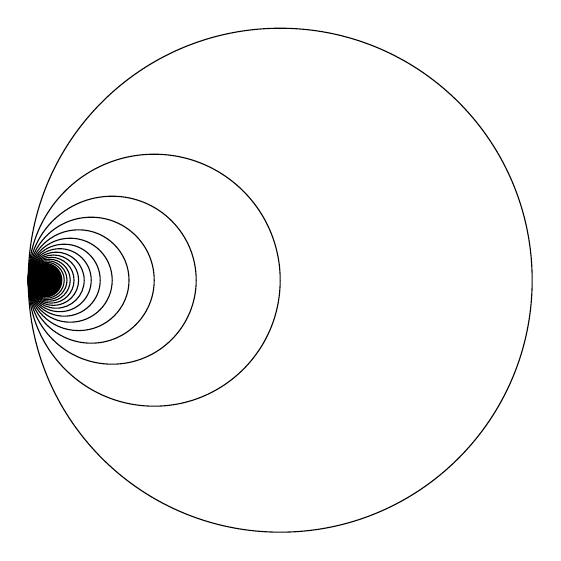
\begin{tikzpicture}[scale=3.2]
  \foreach \n in {1,...,15}{
    \draw ({1/\n},0) circle ({1/\n});
  }
  \fill ({1/15},0) circle ({1/15});
\end{tikzpicture}
\end{document}
